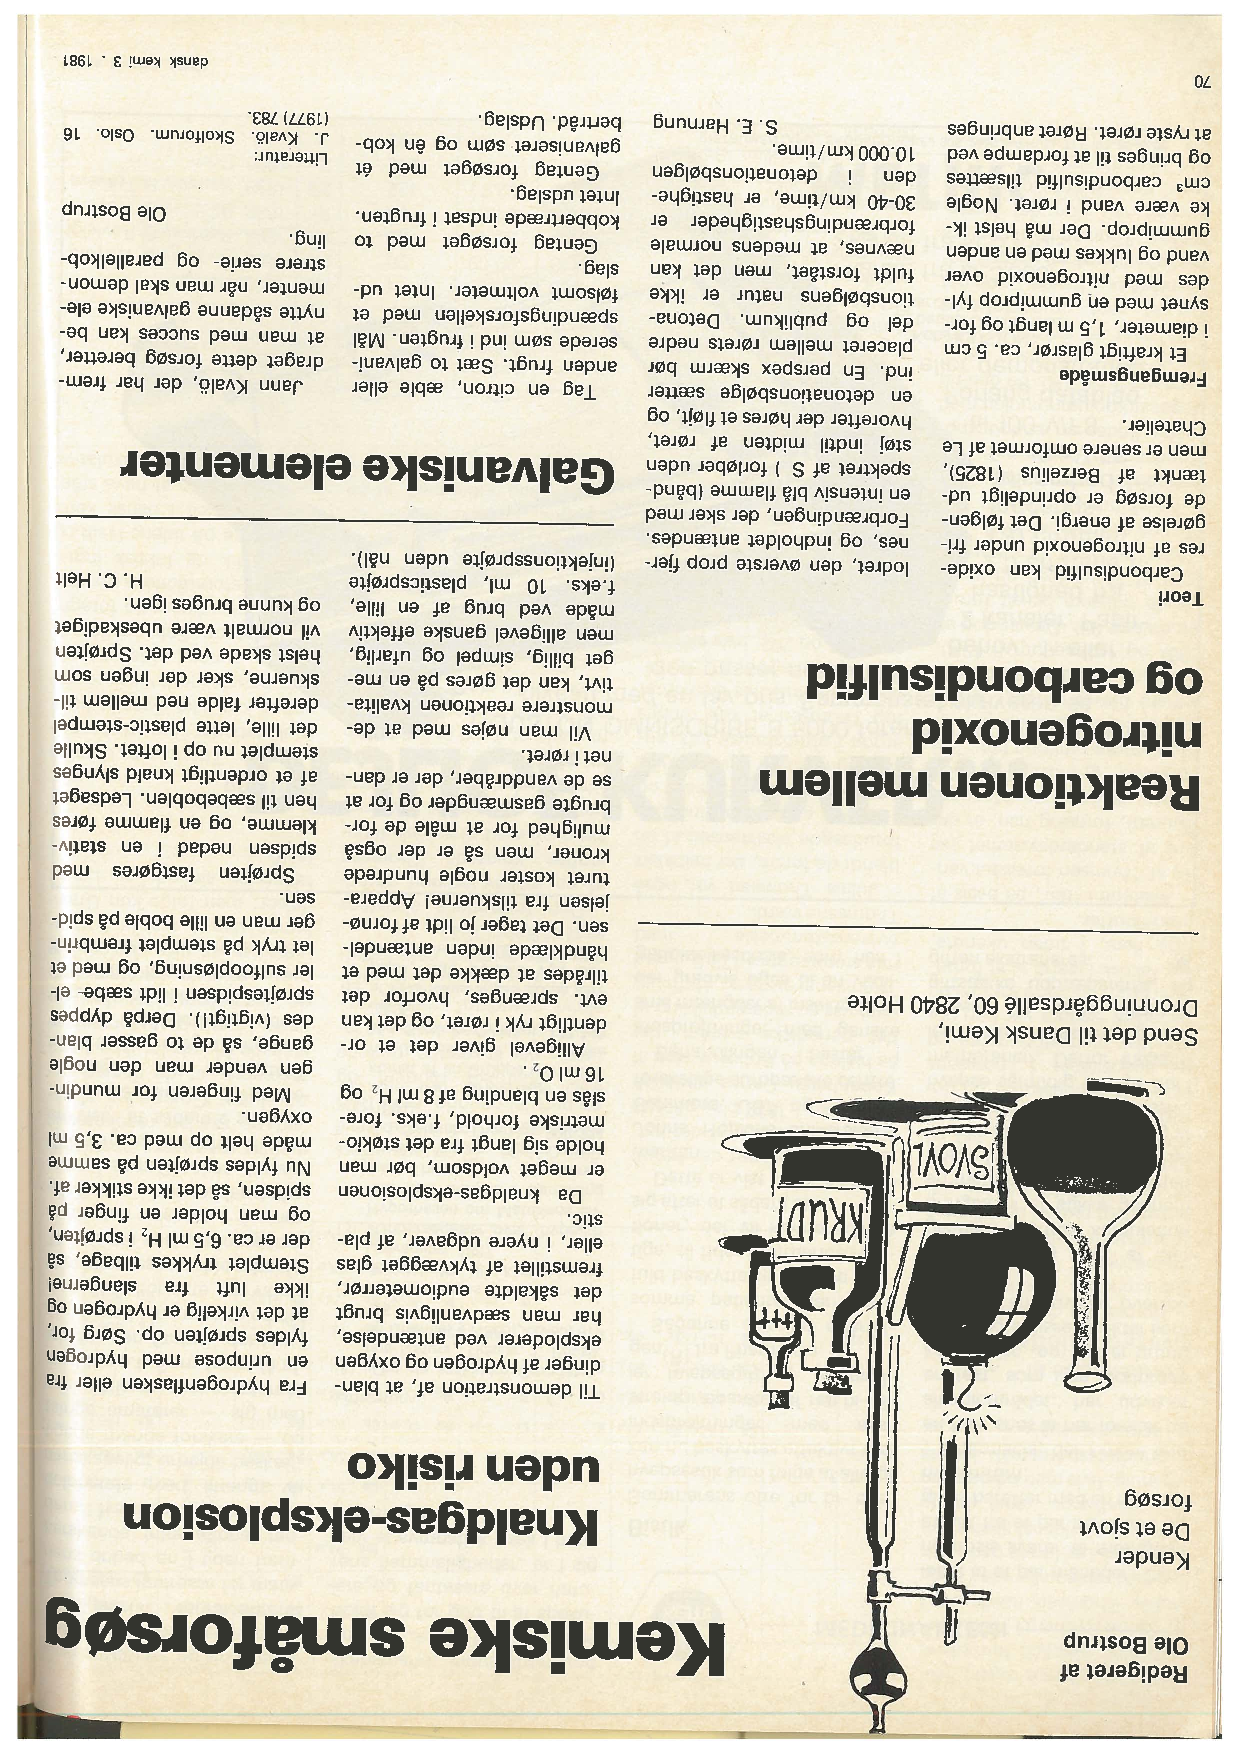
\includepdf[pages=-]{pdfs/1981-62-3-70.pdf}
\danskkemi{Dansk Kemi 62, 3, 1981, p. 70}

Reaktionen mellem nitrogenoxid og carbondisulfid

Forfatter: S. E. Harnung

Teori
carbondisulfid kan oxideres af nitrogenoxid under frigørelse af energi. Det
efterfølgende forsøg er oprindeligt udtænkt af Berzelius (1825), men er
senere omformet af Le Chatelier.

Fremgangsmåde

Et kraftigt glasrør, ca. 5 cm i diameter, 1,5 m langt og forsynet med en gummiprop
fyldes med nitrogenoxid over vand og lukkes med en anden gummiprop.
Der må helst ikke være vand i røret. Nogle cm3 carbondisulfid tilsættes og
bringes til at fordampe ved at ryste røret. Røret anbringes lodret, den
øverste prop fjernes, og indholdet antændes. Forbrændingen, der sker med
en intensiv blå flamme (båndspektret af S) forløber uden støj indtil midten af
røret, hvorefter der høres et fløjt, og en detonationsbølge sætter ind.
En perspex skærm bør placeres mellem rørets nedre del og publikum.
detonationsbølgens natur er ikke fuldt forstået, men det kan nævnes, at
medens normale forbrændingshastigheder er 30-40 km/time, er hastigheden i
detonationsbølgen 10.000 km/time.
